\documentclass[aspectratio=169]{beamer}
\usepackage{color,amsmath}
\usepackage{subfigure}
\usepackage{booktabs}
\usepackage{framed}
\usepackage{comment}
\usepackage{hyperref}
\hypersetup{
    colorlinks=true,
    linkcolor=blue
}
\usepackage{ulem}

%%%%%%%%%%%%%%%%%%%%%%%%%%
\title[]{ TODO }
\author[]{Matthew J. Salganik\\Department of Sociology\\Princeton University}
\date[]{%Summer Institutes in Computational Social Science\\2020
%\vfill
%\begin{flushleft}
%{\scriptsize
%The Summer Institutes in Computational Social Science is supported by grants from the Russell Sage Foundation and the Alfred P. Sloan Foundation.}
%\end{flushleft}
\begin{flushright}

\includegraphics[width=0.1\textwidth]{figures/cc-by.png}
\end{flushright}
}
\begin{document}
%%%%%%%%%%%%%%%%%%%%%%%%%%
\frame{\titlepage}
%%%%%%%%%%%%%%%%%%%%%%%%%%
\begin{frame}

\begin{columns}
\begin{column}{.40\textwidth}
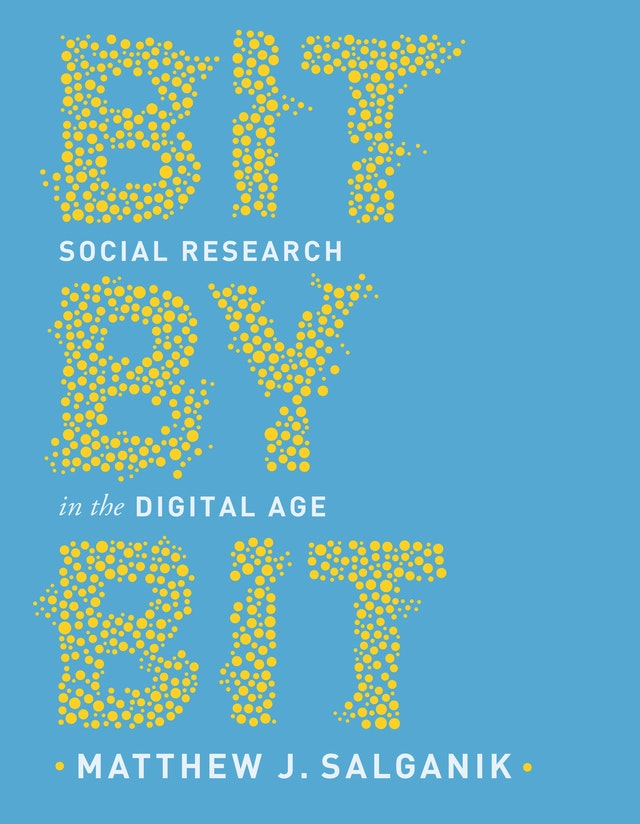
\includegraphics[width=\textwidth]{figures/salganik_bit_2018_cover}
\end{column}%

\hfill%

\begin{column}{.60\textwidth}
1) Introduction \\
2) Observing behavior \\
3) Asking questions \\
4) Running experiments \\
\textcolor{blue}{5) Mass collaboration} \\
6) Ethics \\
7) The future \\
\end{column}%
\end{columns}

\end{frame}
%%%%%%%%%%%%%%%%%%%%%%%%%
\begin{frame}

\begin{center}
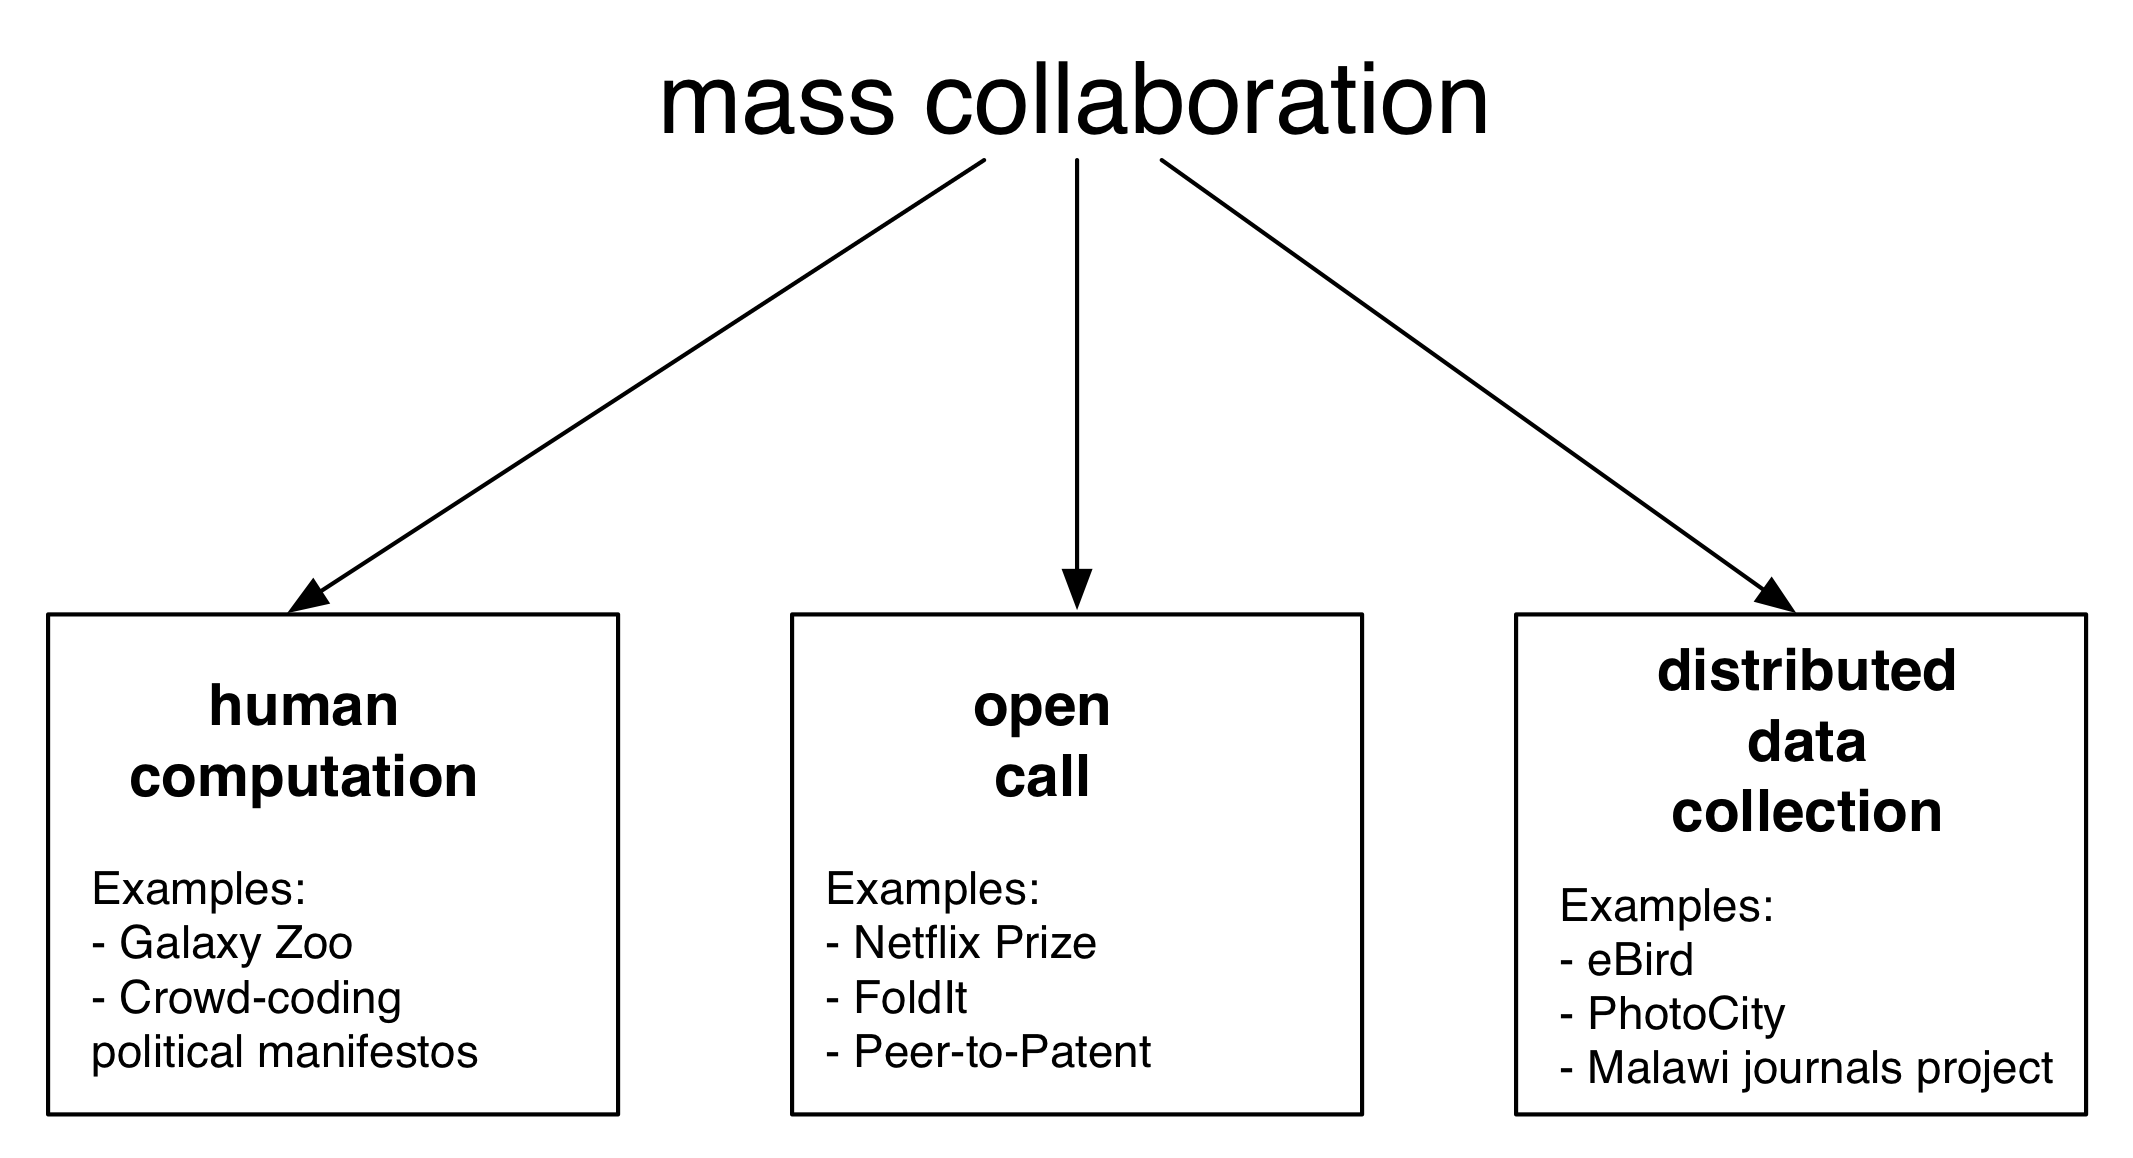
\includegraphics[width=\textwidth]{figures/mass_collaboration_schematic}
\end{center}

\end{frame}
%%%%%%%%%%%%%%%%%%%%%%%%%%
\begin{frame}

\begin{itemize}
\item \textcolor{blue}{Human computation}
\item Open call
\item Distributed data collection
\end{itemize}

\end{frame}
%%%%%%%%%%%%%%%%%%%
\begin{frame}

\begin{itemize}
\item Easy task, big scale
\pause
\item Humans better than computers
\pause
\item Can be combined with supervised learning 
\pause
\item Increasingly important as we move from numeric survey data to working with text, images, movies, audio, etc.
\end{itemize}

\end{frame}
%%%%%%%%%%%%%%%%%%%%%%%%%%

Galaxy Zoo

%%%%%%%%%%%%%%%%%%%%%%%%%%
\begin{frame}

\begin{center}
\only<1>{\includegraphics[width=\textwidth]{figures/benoit_crowd-sourced_2016_title}}
\only<2>{\includegraphics[width=\textwidth]{figures/benoit_crowd-sourced_2016_abstract}}
\end{center}

\vfill
{\tiny \url{http://dx.doi.org/10.1017/S0003055416000058}}

\end{frame}
%%%%%%%%%%%%%%%%%%%%%%%%%%
\begin{frame}

Here's a piece of the manifesto of the Labor Party in the United Kingdom from 2010:

\begin{quote}
``Millions of people working in our public services embody the best values of Britain, helping empower people to make the most of their own lives while protecting them from the risks they should not have to bear on their own. Just as we need to be bolder about the role of government in making markets work fairly, we also need to be bold reformers of government.''
\end{quote}

\end{frame}
%%%%%%%%%%%%%%%%%%%%%%%%%%
\begin{frame}

\begin{center}
\only<1>{\includegraphics[width=\textwidth]{figures/benoit_crowd-sourced_2016_fig1}}
\only<2>{\includegraphics[width=\textwidth]{figures/benoit_crowd-sourced_2016_fig3}}
\end{center}

\end{frame}
%%%%%%%%%%%%%%%%%%%%%%%%%%
\begin{frame}

What I like about Benoit et al (2016)
\begin{itemize}
\item Better not cheaper
\pause
\item Experts are a bug not a feature
\end{itemize}

\end{frame}
%%%%%%%%%%%%%%%%%%%%%%%%%%
\begin{frame}

Wrapping up:
\begin{itemize}
\item Easy task, big scale
\pause
\item Humans better than computers
\pause
\item Can be combined with supervised learning 
\pause
\item Increasingly important as we move from numeric survey data to working with text, images, movies, and audio.
\end{itemize}

\end{frame}
%%%%%%%%%%%%%%%%%%%%%%%%%%
\frame{\titlepage}
%%%%%%%%%%%%%%%%%%%%%%%%%


\end{document}
